\documentclass{article}

\usepackage{fancyhdr} % Required for custom headers
\usepackage{lastpage} % Required to determine the last page for the footer
\usepackage{amsmath}
\usepackage{amsfonts}
\usepackage{graphicx}
\usepackage{subfigure}
\usepackage{listings}
\usepackage{booktabs}
\usepackage[hidelinks]{hyperref}
% \usepackage{epstopdf} uncomment this line if using MiKTeX

% Margins
\topmargin=-0.45in
\evensidemargin=0in
\oddsidemargin=0in
\textwidth=6.5in
\textheight=9.0in
\headsep=0.25in

\linespread{1.25} % Line spacing

% Set up the header and footer
\pagestyle{fancy}
\lhead{\authorName} % Top left header
\chead{\classID\ \hwTitle} % Top center header
\rhead{\studentID} % Top right header
\lfoot{} % Bottom left footer
\cfoot{} % Bottom center footer
\rfoot{Page\ \thepage\ of~\pageref{LastPage}} % Bottom right footer
\renewcommand{\headrulewidth}{0.4pt} % Size of the header rule
\renewcommand{\footrulewidth}{0.4pt} % Size of the footer rule

\setlength{\parindent}{0pt} % Removes all indentation from paragraphs

\setcounter{secnumdepth}{0} % Removes default section numbers
\newcounter{problemCounter} % Creates a counter to keep track of the number of problems

\newcommand{\problemName}{}
\newenvironment{problem}[1][Problem \arabic{problemCounter}]{
	\stepcounter{problemCounter} % Increase counter for number of problems
	\renewcommand{\problemName}{#1} % Assign \problemName the name of the problem
	\section{\problemName} % Make a section in the document with the custom problem count
}{}

\newcommand{\subproblemName}{}
	\newenvironment{subproblem}[1]{
	\renewcommand{\subproblemName}{#1} % Assign \subproblemName to the name of the section from the environment argument
	\subsection{\subproblemName} % Make a subsection with the custom name of the subsection
}{}

%----------------------------------------------------------------------------------------
%	MATH OPERATOR
%----------------------------------------------------------------------------------------

\DeclareMathOperator*{\argmin}{arg\,min}
\DeclareMathOperator*{\argmax}{arg\,max}

%----------------------------------------------------------------------------------------
%	NAME AND CLASS SECTION
%----------------------------------------------------------------------------------------

\newcommand{\hwTitle}{Assignment\ \#2} % Assignment title
\newcommand{\dueDate}{Thursday,\ March\ 10,\ 2015} % Due date
\newcommand{\classID}{ENGG\ 5202} % Course/Class
\newcommand{\authorName}{Kai Chen} % Your name
\newcommand{\studentID}{1155070509} % Your student ID

%----------------------------------------------------------------------------------------
%	TITLE PAGE
%----------------------------------------------------------------------------------------

\title{
	\vspace{2in}
	\textmd{\textbf{\classID:\ \hwTitle}}\\
	\normalsize\vspace{0.1in}\small{Due\ on\ \dueDate}
	\vspace{3in}
}

\author{\textbf{\authorName}}
\date{} % Insert date here if you want it to appear below your name

%----------------------------------------------------------------------------------------

\begin{document}
\maketitle
\setcounter{page}{0}
\thispagestyle{empty}
\newpage

%----------------------------------------------------------------------------------------
%	PROBLEM 1
%----------------------------------------------------------------------------------------

% To have just one problem per page, simply put a \clearpage after each problem

\begin{problem}

\begin{subproblem}{1.1}

\begin{align*}
	l(\theta_1) &= \log p(D_1|\omega_1,\theta_1) \\
	&= \log p(x_{11}|\omega_1,\theta_1) + \log p(x_{12}|\omega_1,\theta_1) \\
	&= 2\log \theta_1 - \theta_1(x_{11}+x_{12})
\end{align*}
Let
\[
	\nabla l(\theta_1) = 0
\]
We get
\[
	\hat{\theta_1} = \frac{2}{x_{11}+x_{12}} = \frac{1}{3}
\]
Similarly,
\[
	\hat{\theta_2} = \frac{2}{x_{21}+x_{22}} = \frac{1}{6}
\]

\end{subproblem}

\begin{subproblem}{1.2}

Given \(\theta_1 = \frac{1}{3}\) and \(\theta_2 = \frac{1}{6}\), we have \\
\[
p(x|\omega_1) =
	\begin{cases}
		0 & x < 0 \\
		\frac{1}{3}\mathrm{e}^{-\frac{x}{3}} & x\geq0
	\end{cases}
\]
\[
p(x|\omega_2) =
	\begin{cases}
		0 & x < 0 \\
		\frac{1}{6}\mathrm{e}^{-\frac{x}{6}} & x\geq0
	\end{cases}
\]
\begin{align*}
	g(x) &= p(\omega_1|x) - p(\omega_2|x) \\
	&= \ln\frac{p(x|\omega_1)}{p(x|\omega_2)} - \ln\frac{p(\omega_1)}{p(\omega_2)}
\end{align*}
Let
\[
	g(x) = 0
\]
We have
\begin{align*}
	x^* &= \frac{\ln\theta_1-\ln\theta_2}{\theta_1-\theta_2} \\
	&= 6\ln2\approx4.16
\end{align*}

\end{subproblem}

\begin{subproblem}{1.3}

The classification rule is when \(x>x^*\), class label is 2, when \(0<x<x^*\), class label is 1. \\
So the expected classification error
\begin{align*}
	Error &= \int_0^{x^*}p(x|\omega_2)p(\omega_2)\mathrm{d}x + \int_{x^*}^\infty p(x|\omega_1)p(\omega_1)\mathrm{d}x \\
	&= \frac{1}{2}\int_0^{6\ln2}\mathrm{e}^{-\frac{x}{6}}\mathrm{d}x + \frac{1}{2}\int_{6\ln2}^\infty\frac{1}{3}\mathrm{e}^{-\frac{x}{3}}\mathrm{d}x \\
	&= \frac{3}{8}
\end{align*}

\end{subproblem}

\end{problem}

%----------------------------------------------------------------------------------------
%	PROBLEM 2
%----------------------------------------------------------------------------------------

\begin{problem}

\(a_{12}\) is updated in the M step and
\begin{align*}
\hat{a}_{12} &= \frac{\sum_{t=2}^T\xi_{t-1}(\omega_1,\omega_2)}{\sum_{t=2}^T\sum_{j'=1}^c\xi_{t-1}(\omega_1,\omega_{j'})} \\
&= \frac{\sum_{t=2}^T P(Z_{t-1}=\omega_1,Z_t=\omega_2|X,\theta^{old})}{\sum_{t=2}^T\sum_{j'=1}^c\xi_{t-1}(\omega_1,\omega_{j'})}
\end{align*}
Because \(a_{12}\) is initialized as 0, therefore for any \(t>1\),we have
\[
	P(Z_{t-1}=\omega_1,Z_t=\omega_2|X,\theta^{old}) = 0
\]
So in all subsequence updates of the EM algorithm \(\hat{a}_{12}=0\).
\end{problem}

%----------------------------------------------------------------------------------------
%	PROBLEM 3
%----------------------------------------------------------------------------------------

\begin{problem}

\begin{subproblem}{3.1}
The sample size for the ``same density'' in \(\mathcal{R}^d\) is \(n_1^d\). \\
If \(n_1=100\), the sample size needed is \(100^{20}\).
\end{subproblem}

\begin{subproblem}{3.2}
\begin{align*}
	p &= \frac{k/n}{V} \\
	  &= k/n \\
	  &= nl_d^d(p)
\end{align*}
So
\[
	l_d(p) = p^\frac{1}{d}
\]
We can calculate
\begin{align*}
l_5(0.01) &= 0.398\\
l_5(0.1) &= 0.63\\
l_{20}(0.1) &= 0.89\\
\end{align*}
\end{subproblem}

\begin{subproblem}{3.3}
If the dimension is high, the edge length of Parzen window will be greater and approximate to 1, leading to larger errors and a ``flat'' and ``uniform'' estimated density.
\end{subproblem}

\end{problem}

%----------------------------------------------------------------------------------------
%	PROBLEM 4
%----------------------------------------------------------------------------------------

\begin{problem}

\begin{subproblem}{4.1}

If it is Gaussian distribution and the class covariances are identical, then the dicision boundary found by two methods will be the same.

\end{subproblem}

\begin{subproblem}{4.2}

The results are shown in table~\ref{tab:4_1} and figure~\ref{fig:4_1}. \\
I observe that LR is more robust than FLD when dealing with outliners and noises. The two algorithms have similar testing error rates when trained using \textbf{train1}, but FLD has significantly larger error rate when trained using \textbf{train1\_2}, because the label of FLD can be infinite while the sigmoid function in LR turns it to (-1, 1), which can handle such outliners.

\begin{table}[!htbp]
\centering
\caption{Dataset 1 results}\label{tab:4_1}
\begin{tabular}{cccc}
\toprule
Train set & Test set & Algorithm & Error rate \\
\midrule
train1 & test1 & FLD & 0.07 \\
train1 & test1 & LR & 0.067 \\
train1\_2 & test1 & FLD & 0.151 \\
train1\_2 & test1 & LR & 0.067 \\
\bottomrule
\end{tabular}
\end{table}

\begin{figure}[htbp]
\centering
\subfigure{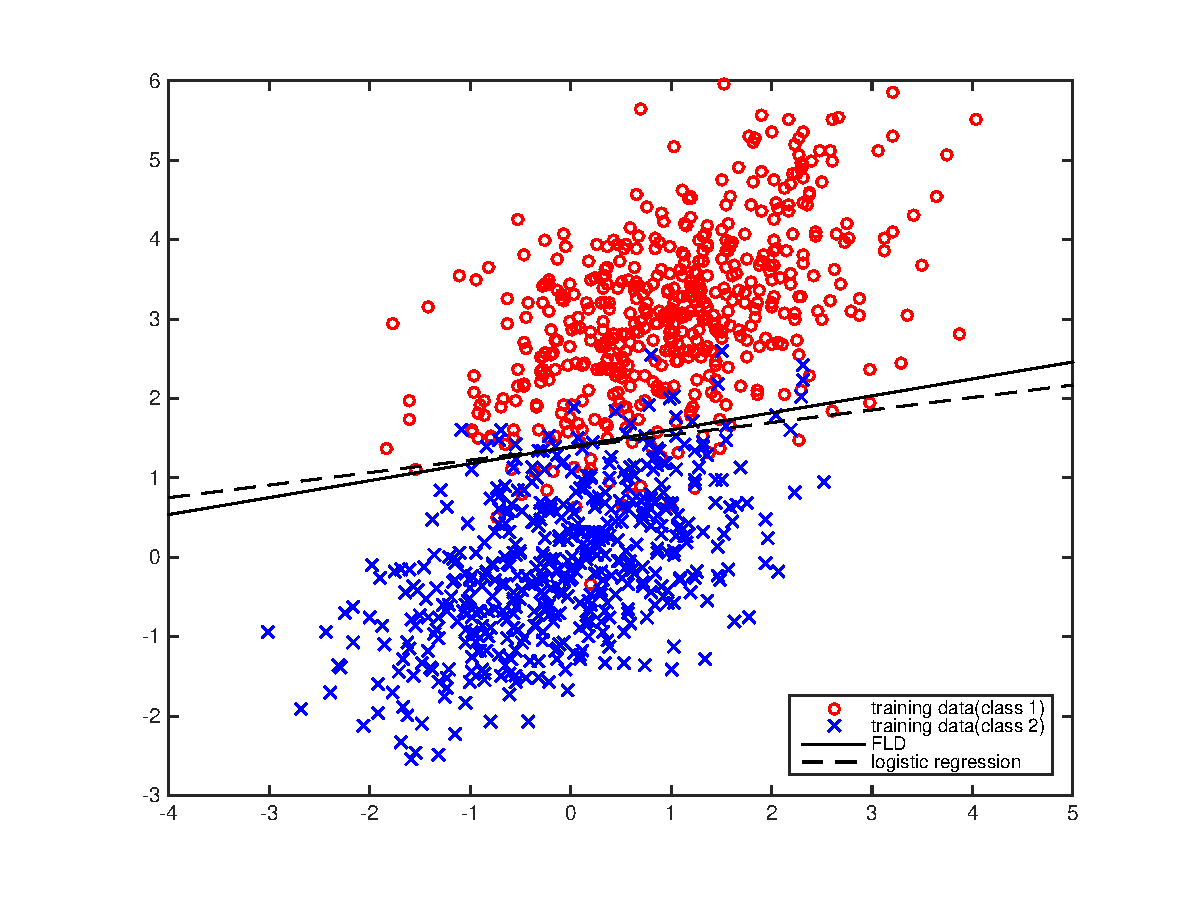
\includegraphics[width=3in]{image/4_1}}
\hspace{0.5cm}
\subfigure{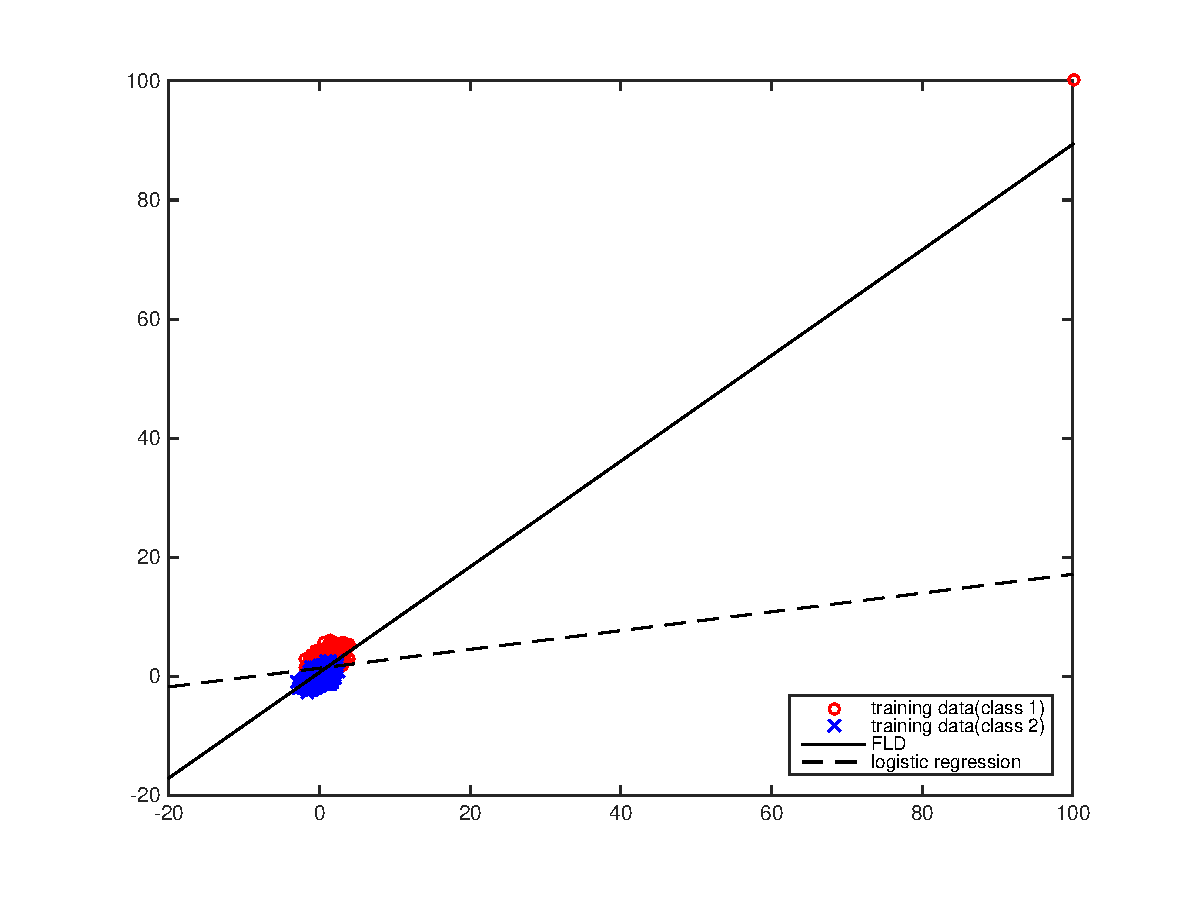
\includegraphics[width=3in]{image/4_2}}
\caption{Train data and decision boundaries (left: train1, right: train1\_2)}\label{fig:4_1}
\end{figure}

\end{subproblem}

\begin{subproblem}{4.3}

The error rates are shown in Table~\ref{tab:4_2}.
The Gaussian asumption is not reasonable for the representation of digit images. The values of \(x\) are discrete and binary, so it is not Gaussian. FLD and LR are sensitive to the Gaussian assumption, because the derivation of these methods are based on Gaussian.

\begin{table}[!htbp]
\centering
\caption{Dataset 2 results}\label{tab:4_2}
\begin{tabular}{cccc}
\toprule
Train set & Test set & Algorithm & Error rate \\
\midrule
train2 & test2 & FLD & 0.23 \\
train2 & test2 & LR & 0.1425 \\
\bottomrule
\end{tabular}
\end{table}

\end{subproblem}

\end{problem}

\end{document}
